
\section{Transport Layer}


\subsection{User Datagram Protocol (UDP)}
{
    \begin{itemize}[noitemsep]
        \item unzuverlässiges, verbindungsloses Protokoll
        \item UDP-Sitzungen werden durch eine 2-Tupel-Adresse (Ziel-IP, Zielport) identifiziert.
        \item  keine Mechanismen zur Fehlererkennung oder Fehlerkorrektur, Zuverlässigkeit und Flusskontrolle
        \item UDP-Pakete $\to$ beliebiger Reihenfolge ankommen oder verloren gehen, ohne  Empfänger benachrichtigt
        \item für Anwendungen:  geringe Latenz $\to$ Echtzeitkommunikation oder Streaming.
        \item Multicasting und Broadcasting, 
    \end{itemize}

}
 
\subsection{Transmission Control Protocol (TCP)}
{

    \begin{itemize}[noitemsep]
        \item zuverlässiges, verbindungsorientiertes Protokoll
        \item implementiert Fehlererkennung, Flusskontrolle und Sequenzierung.
        \item TCP-Sitzungen werden durch eine 4-Tupel-Adresse (Quell-IP, Quellport, Ziel-IP, Zielport) identifiziert.
        \item 3-Way-Handshake, um eine Verbindung aufzubauen: SYN, SYN-ACK, ACK.

        \item  Sequenznummern, um  Reihenfolge empfangener Pakete zu überprüfen und fehlende oder beschädigte Pakete zu erkennen.
        \item Bestätigungen (ACKs), um  Empfang von Datenpaketen zu bestätigen und  Sender informieren, welche Daten erfolgreich übertragen.
        \item Flusskontrolle, um sicherzustellen, dass der Sender Daten nicht schneller sendet, als der Empfänger verarbeiten kann.
        \item Überlastkontrolle, um die Netzwerküberlastung zu vermeiden
        \item Segmentierung von Daten in kleinere Einheiten (Segmenten) für  Übertragung $\to$ stellt sicher, dn Reihenfolge zusammengefügt.
        \item TCP bietet Mechanismen zur Zuverlässigkeit, Flusskontrolle und Fehlerbehebung, ist jedoch im Vergleich zu UDP (User Datagram Protocol) langsamer und erzeugt einen höheren Overhead.
    \end{itemize}
}


\subsection{Ports}
{
    \begin{itemize}[noitemsep]
        \item System Ports (Well-Known)
        \item User Ports (Registered)
        \item Dynamic / Private Ports
    \end{itemize}

    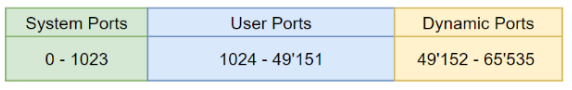
\includegraphics[scale=.45]{img/ports.png}


}


\subsection{Verbindungsauf und -abbau und Datenaustausch}
{
    \begin{tikzpicture}
        \node [examplebox] (box){
            \begin{minipage}{0.3\textwidth}
                { \begin{tabular}{ l l}
                        LISTEN       & Auf Anforderung warten \\
                        SYN-SENT     & Auf Anforderung warten \\
                        SYN-RECEIVED & Anforderung erhalten   \\
                        ESTABLISHED  & Verbindung besteht     \\
                    \end{tabular}}
                \WhiteSpace
                \WhiteSpace
                \begin{tabular}{ l l}
                    SYN & Verbindungsaufbau \\
                    ACK & Paket bestätigen  \\
                    FIN & Verbindungsabbau  \\
                \end{tabular}
                \WhiteSpace
                \WhiteSpace
                \begin{tabular}{ l l}
                    FIN-WAIT-1 & Verbindungsaufbau            \\
                    FIN-WAIT-2 & Abbauanforderung bestätigt   \\
                    CLOSE-WAIT & Auf Lokale Verbindung warten \\
                    LAST-ACK   & Verbindungsabbau bestätigt   \\
                    TIME-WAIT  & Letzte Bestätigung gesendet  \\
                \end{tabular}
            \end{minipage}
        };
        \node[exampletitle, right=8pt] at (box.north west) {Abkürzungen:};
    \end{tikzpicture}

    \begin{tikzpicture}
        \node [examplebox] (box){
            \begin{minipage}{0.3\textwidth}
                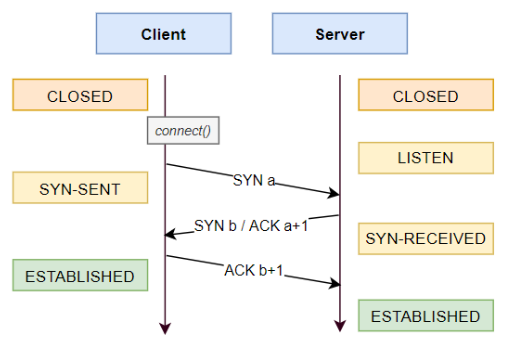
\includegraphics[scale=.45]{img/aufbau.png}
            \end{minipage}
        };
        \node[exampletitle, right=8pt] at (box.north west) {Verbindungsaufbau:};
    \end{tikzpicture}

    \begin{tikzpicture}
        \node [examplebox] (box){
            \begin{minipage}{0.3\textwidth}
                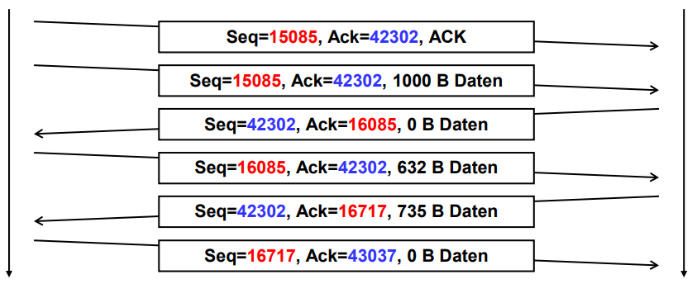
\includegraphics[scale=.35]{img/datenaustausch.png}
            \end{minipage}
        };
        \node[exampletitle, right=8pt] at (box.north west) {Datenaustausch:};
    \end{tikzpicture}


    \begin{tikzpicture}
        \node [examplebox] (box){
            \begin{minipage}{0.3\textwidth}
                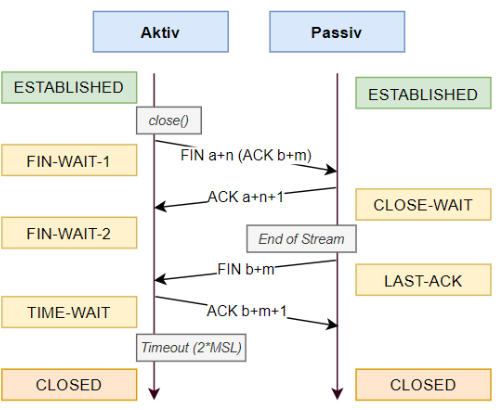
\includegraphics[scale=.45]{img/abbau.png}
            \end{minipage}
        };
        \node[exampletitle, right=8pt] at (box.north west) {Verbindungsabbau:};
    \end{tikzpicture}




}




\subsection{Überlast des Empfängers: Fluss-Steuerung}
{TCP verwendet den Sliding-Window Mechanismus. Beide Seiten einen Buffer (Window).}
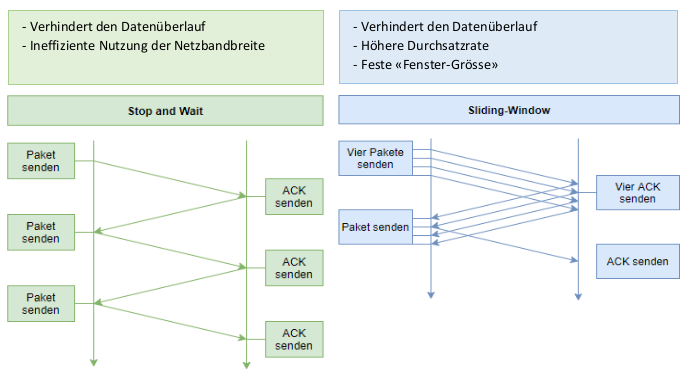
\includegraphics[scale=.375]{img/ueberlast.png}
\subsection{Fluss-Steuerung bei TCP}
{
    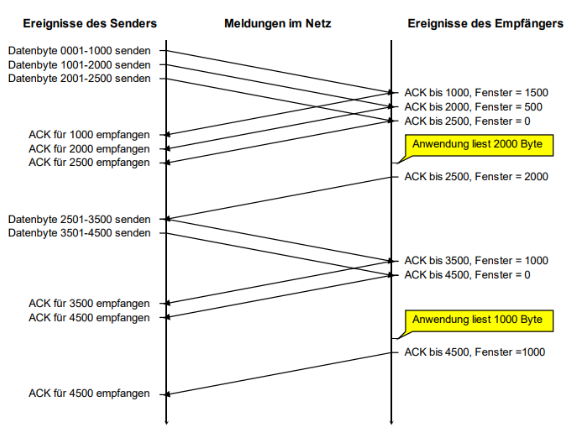
\includegraphics[scale=.45]{img/tcp-flow.png}}

\subsection{Erkennung von verlohrene Telegramme (Round Trip Time)}
{Um Fehler Paketverluste und andere Fehler zu verhindern, werden Pakete nach einer bestimmten Zeit erneut übertragen, wenn keine Bestätigung gesendet wurde.
    Um diese Zeit zu optimieren, misst TCP bei jeder aktiven Verbindung die Round-Trip Time (RTT).}
Retransmission Time-Out RTO